\section{Introduction}

\begin{figure}
 \centering
%  \vspace
 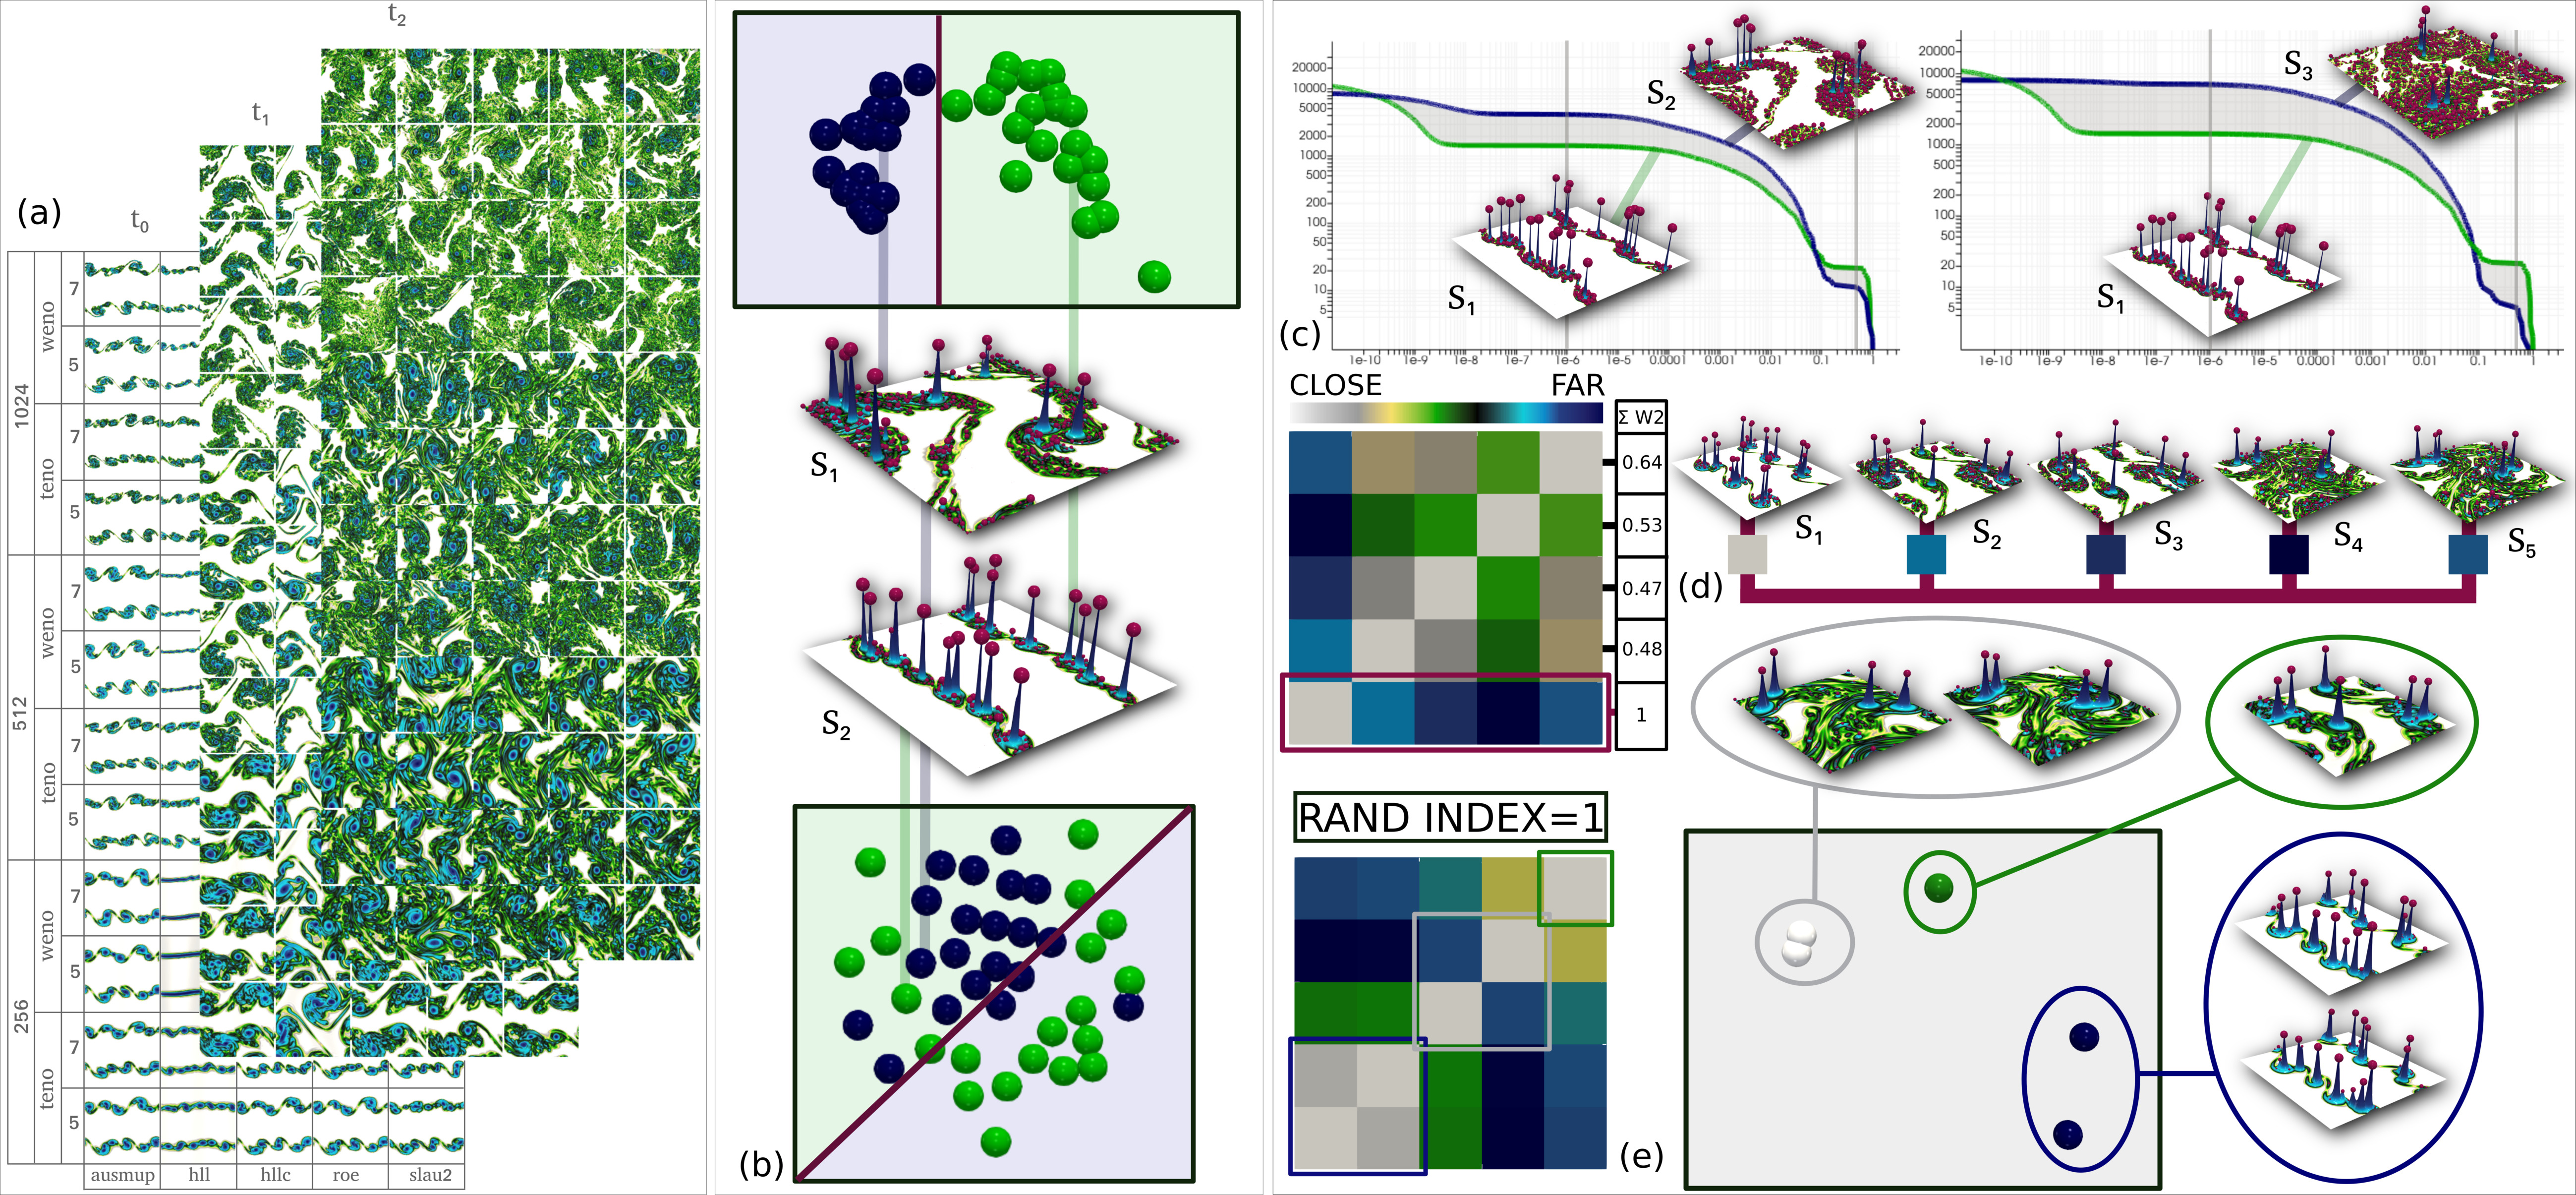
\includegraphics[width=1\linewidth]{chapter4_topology_data_analysis/pictures/teaser2.jpg}
 \caption{ Data Analysis protocols
%   to illustrate the segmentation
applied
  on an ensemble dataset of a Kelvin-Helmholtz instability.
(a) The 180 members of the ensemble obtained with variations of timesteps, interpolation schemes, orders, resolutions and Riemann solvers (\autoref{tab_parameters}).
(b) The top cluster represents the time separation of $t_0$ and $t_1$ for the
flows $S_1$ and $S_2$ with the Wasserstein distance and the bottom cluster with
the $L_2$-norm. Red lines show the timestep separation with our clustering
method whereas the sphere colors are the ground truth, illustrating the
limitation of the $L_2$-norm.
(c) \textit{Persistence curve protocol}: Differences between integrals of persistence curves (gray area) of the enstrophy computed with a SLAU2 solver, an order 7 TENO scheme and a resolution of $1024\times 1024$ for various configurations ($S_1$ at $t_0$, $S_2$ and $S_3$ at $t_1$). These integral differences exhibit the appearance of vortices (critical points) as the time increases.
(d) \textit{Outlier distance protocol}: Wasserstein distance matrix for 5 configurations $S_1(t_0,HLLC)$, $S_2(t_1,Roe)$, $S_3(t_1,HLLC)$, $S_4(t_2,Roe)$, $S_5(t_2,HLLC)$ computed with an order 7 WENO-Z interpolation scheme at $512\times 512$.
The sum of each row
% allows us to identify
the configuration maximizing this distance between solvers and timesteps, here $S_1$.
(e) \textit{Unsupervised classification}: Wasserstein distance matrix for the
previous configurations with an order 7 WENO-Z interpolation scheme at
$256\times 256$. The clustering based on the Wasserstein distance and colored
according to the Kmeans clustering method successfully segments the time
steps.}
 \label{fig_teaser}
\end{figure}

Flow turbulence is a phenomenon of major importance in fluid dynamics.
It is characterized by chaotic changes in the motion of a flow (\emph{e.g.}
typical cigarette smoke patterns), which have a drastic impact in numerous
applications (aeronautics, weather forecast, climate modeling, material
sciences, astronomy, etc.).
Although turbulence has been studied since the early stages of modern physics,
its theoretical mastery remains incomplete \cite{baez2006} and the
understanding of the
Navier-Stokes equations, central
in the description of
% to
fluid motion, is still
considered as
a
% one of the
major open challenge in mathematics and physics,
as proven by the Clay Mathematics Institute selecting it to be
% and
% has been selected by
among its celebrated Millennium Prize problems \cite{fefferman2000}.
Thus, in engineering applications, the main practical solution available for
the study of turbulence
% and turbulent flows
remains numerical simulation.

\noindent
\textbf{Problem introduction:}
However,
% plenty of
many
different numerical solvers can be used to simulate a given flow configuration, each
solver being itself subject to several input parameters (such as domain
resolution, interpolation scheme and order, etc.): when faced with such a wide variety,
% \julien
the main problem for users becomes
the configuration itself of the simulation parameters.
% to choose the right solver.
% Then, the problem of evaluating and comparing the performance of different solver configurations is
% of major importance.
In particular, domain experts want not only to identify
the solver configurations which produce the most realistic simulations, but
they also want to discover configurations resulting in
degraded but fast
% fast, degraded
computations, which still produce simulations of acceptable realism. The
fundamental problem behind such comparative analyses is that of comparing
\emph{quantitatively} turbulent flows. For instance, the quantitative realism
of a simulation could be evaluated by comparing its outcome to a reference,
either obtained by acquisition or by a highly detailed simulation considered as
a ground-truth. However, the chaotic nature of turbulent flows makes their direct
comparison with standard imaging tools
% (\emph{e.g.} the $L_2$ norm, \autoref{fig_teaser})
impractical. For instance, turbulent flows which are considered similar at a
high level by domain experts (in terms of the number and size of their vortices)
are reported by classical metrics such as the $L_2$ norm as being very distant
(\autoref{fig_teaser}), as such pointwise measures are sensitive to mild
geometrical variations in the data and miss global structural
similarities in such a chaotic context. This observation motivates the
consideration of alternative similarity estimation tools, which focus on the
\emph{structure} of the flow, rather than its raw geometry.

In that regard, Topological Data Analysis (TDA) \cite{edelsbrunner09} forms a
family of generic, robust and efficient techniques, whose purpose is precisely
to recover hidden implicit structural patterns in complex data, and to enable
their reliable representation and comparison. As such, they provide
potentially relevant alternatives to standard comparison measures used in
scientific imaging, such as the $L_2$ norm. Moreover, the utility of TDA has
been already demonstrated in a number of analysis and visualization tasks
\cite{heine16}, with examples of successful applications in
combustion \cite{laney_vis06, bremer_tvcg11, gyulassy_ev14},
material sciences \cite{gyulassy_vis07, gyulassy_vis15, favelier16},
% fluid dynamics \cite{kasten_tvcg11},
bioimaging \cite{carr04, topoAngler, beiBrain18},
quantum chemistry \cite{chemistry_vis14, harshChemistry, Malgorzata19}, or
astrophysics \cite{sousbie11, shivashankar2016felix}. In
particular, the critical points of flow vorticity indicators have been
reported to appropriately capture the center of vortices \cite{kasten_tvcg11,
bridel_ldav19}, as well as their importance, with the notion of
\emph{topological persistence} \cite{edelsbrunner02}. Such  results provide
additional evidence and consolidate the intuition that TDA could be a
relevant framework for comparing turbulent flows.

The ambition of this application paper is to provide a comprehensive
experimental evaluation of
% experimentally
% evaluate
the above intuition, i.e. to assess the suitability of
topological data representations and their associated analysis tools for the
quantitative comparisons of turbulent flows.
%We shall focus on a peculiar type of turbulence that expresses itself in two dimensions (akin to the soap-film turbulence displayed in Fig.~\ref{fig:soapfilm}): it is a fair representative of generic turbulence (\emph{a.k.a.} three-dimensional viscous turbulence) and allows for affordable high-resolution simulations to feed our study.
We shall focus on a specific type of turbulence that expresses itself in two dimensions (Kelvin-Helmholtz instability): it is a fair representative of generic turbulence (\emph{a.k.a.} three-dimensional viscous turbulence) and allows for affordable high-resolution simulations to feed our study.
% Image du SAVON
%\begin{figure}
%    \centering
%    \includegraphics[width=0.75\linewidth]{turbulenceinasoapfilm_cut.jpeg}
%    \caption{Experimentally generated, gravity-driven, turbulent soap film.Interference fringes in yellow light (wavelength = 0.589 µm) make it possible to visualize the generation of 2D turbulence\cite{tran2010macroscopic}.Color-reproduction courtesy of Okinawa Institute of Science and Technology.}
%\label{fig:soapfilm}
%\end{figure}
Specifically, our study documents
the usage of the persistence diagram of the maxima of flow enstrophy (an established indicator of vorticity for two-dimensional flows,
\autoref{sec_background}) for the topological representation of 180 members of
an ensemble of hydrodynamic turbulent flows, generated by a coarse sampling of
the parameter space of five distinct solvers.
We document five main hypotheses (\autoref{sec_caseStudy}) reported by domain
experts, describing their expectations with regard to the variability among the
flows generated by the distinct solver configurations.
Then, we describe three evaluation protocols (\autoref{sec_protocols}) designed
to assess the validation of the above hypotheses by standard comparison
measures ($L_2$ norm) on one hand, and by topological methods on the other.
Specifically, these protocols exploit the persistence curve, the
$L_2$-Wasserstein distance between persistence diagrams \cite{Turner2014} and
$k$-means in the $L_2$-Wasserstein metric space \cite{vidal_vis19}. Finally, we
document
the
results of these
% evaluation
protocols on the input ensemble
% , are
% documented
% and the corresponding insights are discussed
(\autoref{sec_experimentalResults}). We believe that the insights reported by
our study bring a strong experimental evidence of the suitability
of TDA for representing and comparing turbulent flows, thereby providing
confidence in its usage by the fluid dynamics community in the future.
Moreover, our flow data and evaluation protocols provide to the TDA community
an application-approved benchmark for the evaluation and design of further
topological distances in the future.

% can be used as a justification in future work.

% While several, global indicators are
% established in the computational fluid dynamic community (such as energy plots
% as function of wave numbers, \autoref{sec_relatedWork})

% \julien{One sentence to explain why they are difficult to study.}
% \julien{One sentence explaining the vast possibilities in terms of solver
% and parameters and the difficulty to tune them.}
% \julien{One sentence explaining that existing quality metrics and their
% limitations: they are global, they don't take into account subtle behaviors,
% this is a problem when increasing the resolutions because vortices have a
% very restricted spatial support (hence their contribution impact modestly
% aggregative quality metrics).}
% \julien{One sentence to explain that two ensemble members are rather hard to
% compare, since two similar flows from a fluid mechanics point of view, can be
% highly dissimilar visually, which challenges standard metrics such as the $L_2$
% norm. This motivates more advanced tools capable of extracting features of
% interest and compare them directly.}
% \julien{One sentence to announce that in this work, we perform an exhaustive
% experimental study to evaluate the relevance of topological data
% representations for the evaluation and comparisons of solvers of hydrodynamic
% turbulent flows.}
% \julien{One sentence to explain quickly what topological data representations
% are about and in which context they have been used. Finish on recent work
% suggesting to compare them and study them at a statistical level. We exploit
% these recent advances in our current work.}
% \julien{Brief overview of the kinds of study we're going to show
% (\autoref{sec_protocols}): (i) comparisons of persistence curves, (ii)
% Wasserstein distances between persistence diagrams, (iii) Clustering in the
% Wasserstein metric space.}
% \julien{An exhaustive analysis on an ensemble of 180 members
% \autoref{sec_experimentalResults} validate the ability of topological
% descriptors to discriminate better different regions parameter space, and
% reveal  new insights on hydrodynamic turbulent flow simulations.}

% \vspace{-1ex}
\begin{figure}
 \centering
%  \vspace
 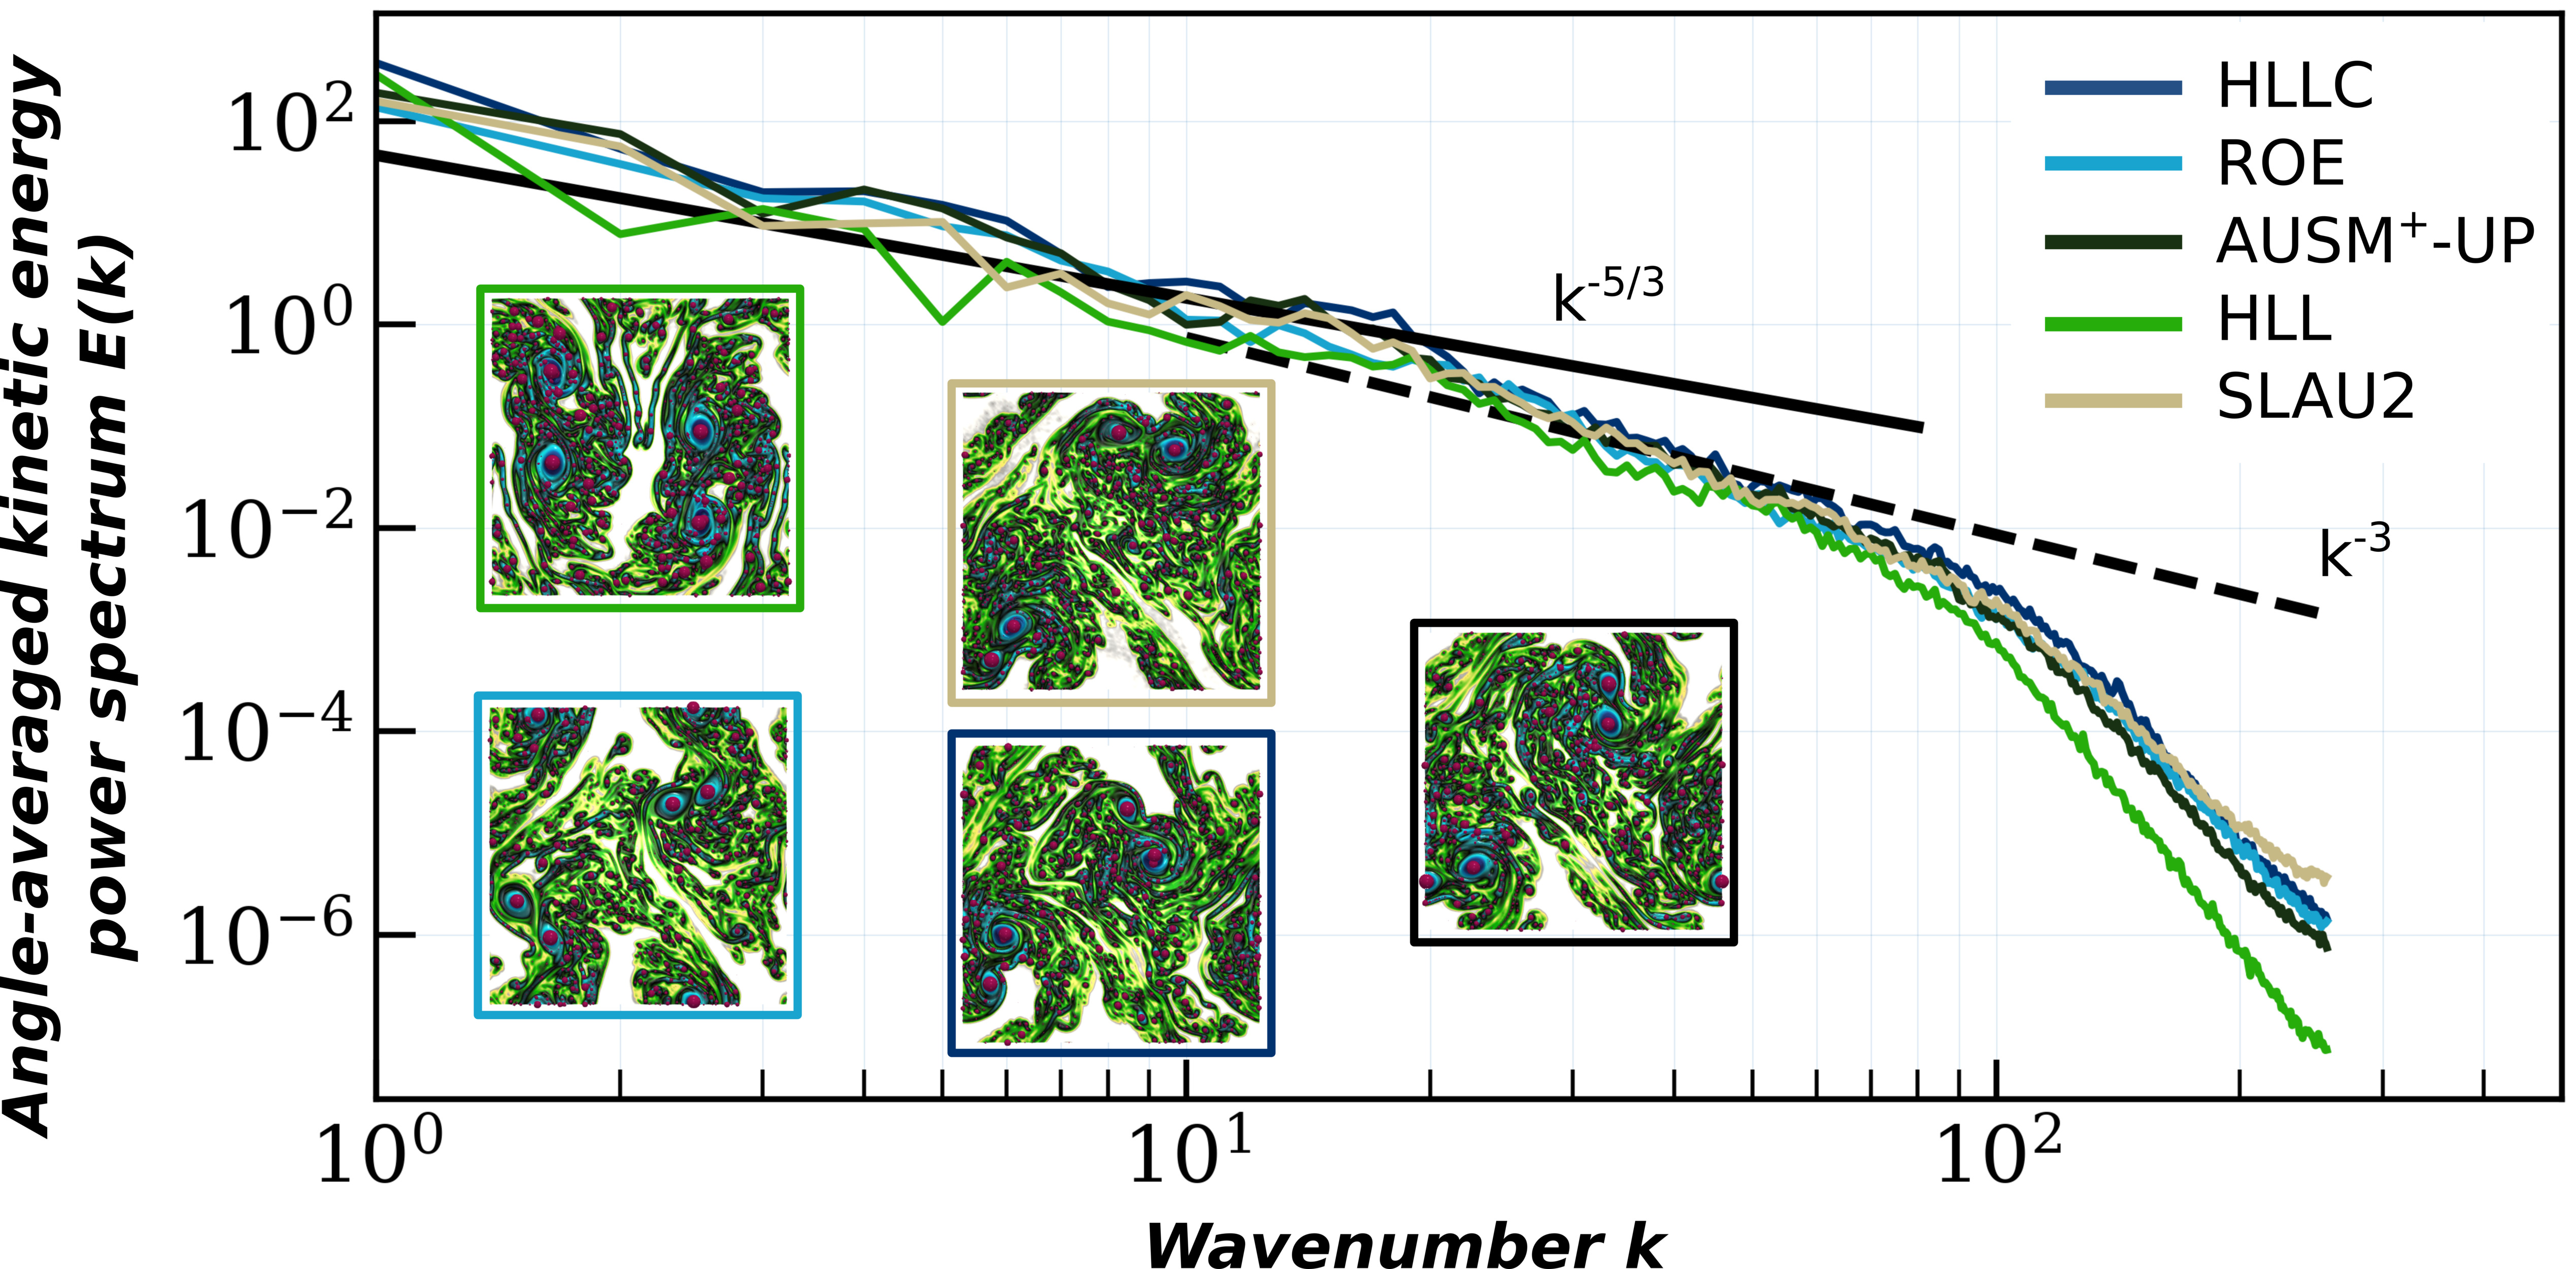
\includegraphics[width=\linewidth]{chapter4_topology_data_analysis/pictures/energie.jpg}
 \mycaption{Baseline analysis by angle-averaged kinetic energy power spectrum
 for all solvers (WENO-Z, order $7$, $t_2$, $512\times512$).
%  with the WENO-Z seventh order, at $t_2$, with 512 x 512 cells for all solvers.
 }
 \label{energie}
\end{figure}

\subsection{Related work}
\label{sec_relatedWork}
This section presents the literature related to our work.
First, we
 discuss previous work dealing with \emph{(i)} simulations of turbulent
flow
% as well as
and their quantitative evaluation. Next, \emph{(ii)} we review
previous work dealing with topological methods for the analysis of ensemble
data.

\noindent
\textbf{\emph{(i)} Turbulent flow simulation.}
% \julien{todo:
% \begin{enumerate}
%  \item Faire un bref historique des références clés pour la simulation
% d'écoulements turbulents
%  \item Faire un bref historique des méthodes clés pour évaluer quantitativement
% la qualité d'un écoulement.
% \end{enumerate}
% }
Turbulence is ubiquitous in nature, at all scales, from Higgs-Boson condensates \cite{Kraichnan1967} to a stirred cup of coffee to geophysical flows \cite{Kraichnan1980} to galaxy formation.
While a significant literature in graphics \cite{KimTJG08, ZhangLSSQ14, BaiWDL21} focused on the efficient generation of visually plausible turbulence, we focus in this work on the direct numerical simulation of the underlying physical equations, for engineering applications.
% One motivation to study turbulence, and in particular two-dimensional turbulence, shared by all investigators is that despite its practical applications, its omnipresence and the years of scrutiny it was subjected to, remains one of the most important unsolved problems of classical mechanics.
A special distinction of 2D turbulence is that it is never realized in nature that, unless strongly constrained,
%\cite{Danilov2002},
always has some degree of three-dimensionality but rather it only exists in computer simulations.
Two-dimensional turbulence has thus been studied extensively by the latter means \emph{e.g.} for its importance as an idealization of meteorological flows \cite{Boffetta2011}, its role in the confinement of thermonuclear plasmas \cite{Kraichnan1980} but also as a cost-effective numerical testing ground for three-dimensional flows dynamical theories \cite{Tabeling2002}.
Most such studies focus either on validating predictions of theorists \cite{Kraichnan1967,lilly1989two} or on providing insights into the dynamic behavior of 2D eddies thanks to high-resolution simulations \cite{lilly1989two,Maltrud1991}.
The simulations are usually analyzed by considering macroscopic quantities such as the enstrophy (see below equation~\eqref{eq:enstrophy}), or by considering the Fourier decomposition of the 2D field (similar to \autoref{energie})- integral indicators that make it near impossible to compare and/or classify the results of, say, a parametric study.
% These classical indicators all integrate the data to some extent and, faced with two numerical realizations produced using different numerical settings, make it near impossible to classify the results.
Some efforts have been made recently \cite{san2015evaluation} to provide the users with some guidelines to best choose the numerical methods and parameters for the simulation of 2D turbulence, but still using, mostly, the aforementioned integral, inaccurate, indicators.
The present study aims at providing the workers in 2D turbulence with another tool to classify their results and best choose their settings, this time using mostly local indicators able to exploit the whole flow.

\noindent
\textbf{\emph{(ii)} Topological methods for ensemble analysis.}
Concepts and algorithms from computational topology \cite{edelsbrunner09} have
been investigated, adapted and extended by the visualization community for more
than twenty years \cite{heine16}. Specifically, a large body of literature has
been dedicated to the analysis and visualization of flow data with
topological methods and we refer the readers to a series of surveys on the topic
\cite{ScheuermannT05, GarthT06,
LarameeHZP07, PobitzerPFSKTMH11,
wang2016,
BujackYHGW20},
including a
recent iteration \cite{flowIntro21}.
A substantial line of work
\cite{petz, otto2, otto1} focused on extending topological techniques to
uncertain vector fields, where flow variability is encoded via a pointwise
estimator (\emph{e.g.} an histogram) of an \emph{a priori} vector distribution, but only few
techniques explicitly focused on the analysis of flow variability in an
ensemble.
Specifically, several comparative visualization techniques have been
proposed \cite{filip3, schneider2012,Hummel2013, GuoHPSCH16, JaremaKW16, filip2, filip1, LohfinkG20}. Ferstl et al.
\cite{Ferstl2016} investigated the global structure of flow ensembles, by
proposing a  clustering approach of the  members, based on a measure of
streamline similarity.
However, these techniques assume a mild
geometrical variability within the ensemble and are therefore
% are
not suited to highly
turbulent flows as studied in this work, where the geometry of the features
(streamlines, vortices) chaotically changes from one ensemble
member to the other (\autoref{fig_teaser}), even upon only slight variations of
the simulation input parameters.
In certain application contexts, CFD experts often prefer to focus their analysis on (simpler to interpret) scalar descriptors generated from the flow, such as the kinetic energy (\autoref{energie}) or the enstrophy (\autoref{eq:enstrophy}). Such a transition to a scalar descriptor enables them to leverage the existing tools for scalar data analysis.
% In several applications, the features of interest in the flow can be reliably
% represented by considering a single pointwise scalar descriptor, such as
% pressure, energy or an estimation of vorticity for instance.
% Such a transition to a scalar descriptor of the flow enables users to leverage
% the ensemble of existing tools for scalar data analysis.
For instance, several
authors \cite{kasten_tvcg11, bridel_ldav19} have shown that, given a relevant
vorticity scalar descriptor, the center of the flow vortices could be reliably
extracted and tracked over time, which supports the idea that
topological methods for scalar data can be useful for the description of
specific flow features. Thus, in the following, we describe the literature
related to topological methods for scalar data.
Popular topological representations include the persistence diagram
\cite{edelsbrunner02, edelsbrunner09}
% (\autoref{fig_mergeTree}),
which represents the
population of features of interest in function of their salience, and which
can be computed via matrix reduction
\cite{edelsbrunner09, dipha}. The Reeb graph \cite{biasotti08}, which describes
the connectivity evolution of level sets, has also been widely studied and
several efficient algorithms have been documented \cite{pascucci07,
tierny_vis09, parsa12, DoraiswamyN13}, including parallel algorithms
\cite{gueunet_egpgv19}.
Efficient algorithms have also been documented for its variants,
% including
the
merge and contour trees \cite{tarasov98, carr00}
and parallel algorithms have
also been described \cite{MaadasamyDN12, AcharyaN15,
CarrWSA16, gueunet_tpds19}. The Morse-Smale complex \cite{EdelsbrunnerHZ01,
EdelsbrunnerHNP03,
BremerEHP03}, which depicts the
global behavior of integral lines, is another popular topological data
abstraction in visualization \cite{Defl15}. Robust and efficient algorithms
have been introduced for its computation  \cite{robins_pami11, ShivashankarN12,
gyulassy_vis18} based on Discrete Morse Theory \cite{forman98}.
Inspired by the literature in
optimal transport \cite{Kantorovich, monge81}, the Wasserstein distance between
persistence diagrams \cite{edelsbrunner09}
(and its variant the
Bottleneck distance \cite{edelsbrunner02}) have been extensively studied.
% This distance
% is based on a bipartite assignment problem.
In
practice, it enables users to compare ensemble members based on their
persistence diagrams.
In our experimental study, we focus on this first, established topological tool
for comparing the topology of ensemble members and we refer the reader to a
recent survey \cite{YanMSRNHW21} for a description of alternative metrics
between topological descriptors.
Several techniques have been proposed for summarizing the topological features
in an ensemble or analyzing their variability.
% For instance,
Favelier et al.
\cite{favelier2018} and Athawale et al. \cite{athawale_tvcg19} introduced
approaches for analyzing the variability of critical points and
gradient separatrices respectively. Recent approaches aimed at summarizing
an ensemble of topological descriptors by computing a notion of \emph{average}
% topological
descriptor,
% with respect to
given a specific metric.
% Such a
This notion has
been well studied for persistence diagrams \cite{Turner2014,
lacombe2018, vidal_vis19}, with direct applications to ensemble clustering
\cite{vidal_vis19}, and analogies have been developed for merge
trees \cite{YanWMGW20, pont_vis21}.
%
% - scalar data ensemble analysis (cite previous work on ensemble)
% % (\autoref{sec_background_persistenceDiagrams}),
% % for which exact
% % \cite{Munkres1957} and approximate \cite{Bertsekas81, Kerber2016}
% % implementations are publicly available \cite{ttk17}.
%
% These building blocks have been well studied
% for persistence diagrams
% barycenters of diagrams
% \cite{Turner2014,
% lacombe2018, vidal_vis19}.
% analogies recently developed for merge trees \cite{YanWMGW20, pont_vis21}.
%
%
% \julien{Related work in topology, applications to various fields including flow
% analysis.}

% \fabien{Test}
% \florent{Test2}


\subsection{Contributions}
This application paper makes the following new contributions:
\vspace{-1ex}
\begin{enumerate}[itemsep=-0.75ex]
 \item{\emph{An evaluation procedure for distances between turbulent
flows:}
 We document 5 main hypotheses reported by domain experts, describing their
expectations
about
% regarding
flow variability
within the studied ensemble (180 members).
We contribute 3 evaluation protocols,
to assess
the validation of the
hypotheses by a specific metric,
given as a distance matrix between the members;}
 \item{\emph{A comprehensive experimental study:}
 We provide a detailed experimental study of the ensemble under consideration
for two distance metrics: \emph{(i)} a standard distance used in scientific
imaging (the $L_2$ norm) and \emph{(ii)} an established topological distance
between persistence diagrams (the $L_2$-Wasserstein metric). Our
experiments demonstrate the superiority of the topological distance to report
as close solver configurations which are expected to be similar by domain
experts. The insights reported by our study bring an experimental evidence
of the suitability of the persistence diagram for representing and comparing
turbulent flows, thereby providing to the fluid dynamics community confidence
for its usage in future work;}
 \item{\emph{An application-approved benchmark:}
 We provide as supplemental material \emph{(i)} the input ensemble of 180
turbulent flows (see \cite{data} for a direct link)
% as well as
and
%\emph{(ii)} Python scripts for reproducing our results.
%Our scripts support the usage of custom distance matrices, thereby providing to the TDA community an application-approved benchmark for the evaluation and design of further topological distances.
\emph{(ii)} a python template script for reproducing our results.
Our script supports the usage of custom distance matrices, thereby providing to
the TDA community an application-approved template for the evaluation and design
of further topological distances.
}


\end{enumerate}

